\subsubsection{Deleting Edge from an Internal Node}\label{Subsubsec: Deleting Edge from an Internal Node}

\begin{figure}[H]
    \centering
    \begin{subfigure}{0.45\textwidth}
        \centering
        \begin{tikzpicture}[->,shorten >=1pt,auto,node distance=2cm,
            thick,main node/.style={circle,draw,font=\sffamily\bfseries}]

        % Define vertices
        \node[main node] (4) {$4_{in}$};
        \node[main node] (44) [left of=1] {$4_{out}$};
        \node[main node] (6) [below of=1] {6};
        \node[main node] (8) [below of=11] {8};
        

        % Draw edges
        \path[every node/.style={font=\sffamily\small}]
            (44) edge (8)
            (8) edge (6)
            (6) edge (4);

        \end{tikzpicture}
        \caption{Graph in Tree Node B}
        \label{fig:tree_node_b_graph}
    \end{subfigure}
    \hfill
    \begin{subfigure}{0.45\textwidth}
        \centering
        \begin{tikzpicture}[->,shorten >=1pt,auto,node distance=2cm,
            thick,main node/.style={circle,draw,font=\sffamily\bfseries}]

        % Define vertices
        \node[main node] (4) {$4_{in}$};
        \node[main node] (44) [left of=1] {$4_{out}$};
        \node[main node] (6) [below of=1] {6};
        \node[main node] (8) [below of=11] {8};
        

        % Draw edges
        \path[every node/.style={font=\sffamily\small}]
            (8) edge (6)
            (6) edge (4);

        \end{tikzpicture}
        \caption{Graph after deleting edge 4 to 8}
        \label{fig:graph_after_dedge_4_to_8}
    \end{subfigure}
    \caption{Graph in Tree Node B after deleting edge 4 to 8}
    \label{fig:tree_node_b_graph_after_dedge1}
\end{figure}

\begin{figure}[H]
    \centering
    \begin{subfigure}{0.45\textwidth}
        \centering
        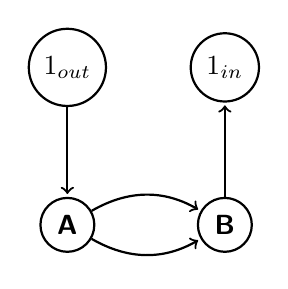
\begin{tikzpicture}[->,shorten >=1pt,auto,node distance=2cm,
            thick,main node/.style={circle,draw,font=\sffamily\bfseries}]

        % Define vertices
        \node[main node] (1) {$1_{in}$};
        \node[main node] (11) [left of=1] {$1_{out}$};
        \node[main node] (A) [below of=11] {A};
        \node[main node] (B) [below of=1] {B};
        

        % Draw edges
        \path[every node/.style={font=\sffamily\small}]
            (11) edge (A)
            (A) edge[bend left] (B)
            (A) edge[bend right] (B)
            (B) edge (1);

        \end{tikzpicture}
        \caption{Graph in SCC Tree Node R}
    \end{subfigure}
    \hfill
    \begin{subfigure}{0.45\textwidth}
        \centering
        \begin{tikzpicture}[->,shorten >=1pt,auto,node distance=2cm,
            thick,main node/.style={circle,draw,font=\sffamily\bfseries}]

        % Define vertices
        \node[main node] (1) {$1_{in}$};
        \node[main node] (11) [left of=1] {$1_{out}$};
        \node[main node] (A) [below left of=11] {A};
        \node[main node] (8) [below right of=A] {8};
        \node[main node] (6) [right of=8] {6};
        \node[main node] (4) [above right of=6] {4};
        

        % Draw edges
        \path[every node/.style={font=\sffamily\small}]
            (11) edge (A)
            (A) edge[bend left] (8)
            (A) edge[bend right] (8)
            (8) edge (6)
            (6) edge (4)
            (4) edge (1);

        \draw [red, rounded corners, dashed] ($(8) + (-0.5 , 0.5)$) -- ($(6) + (0,0.5)$) -- ($(4) + (-0.5, 0)$) -- ($(4) + (-0.5, 0.5)$) -- ($(4) + (0, 0.5)$) -- ($(4) + (0.5, 0.5)$) -- ($(4) + (0.5, 0)$) 
        -- ($(4) + (0.5, -0.25)$) -- ($(6) + (0.25, -0.5)$) -- ($(8) + (-0.5, -0.5)$) -- cycle;
        \end{tikzpicture}
        \caption{After Exposure}
        \label{fig:tree_node_r_graph_exposed1}
    \end{subfigure}
    \caption{Graph in SCC Tree Node R after unreachable nodes and its corresponding edges are exposed}
\end{figure}

\begin{figure}[H]
\centering
\begin{subfigure}{0.45\textwidth}
    \centering
    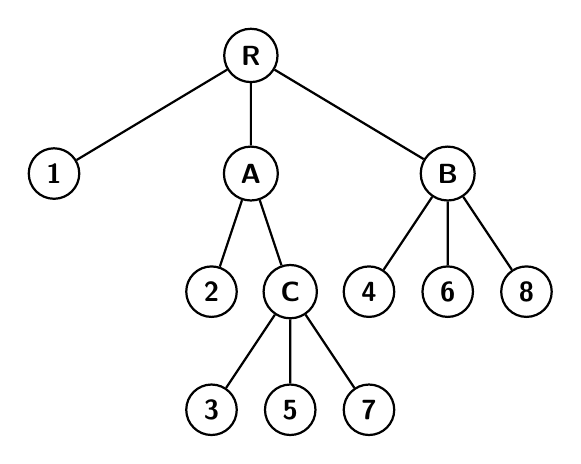
\begin{tikzpicture}[level distance=1.5cm,
                        level 1/.style={sibling distance=2.5cm},
                        level 2/.style={sibling distance=1cm},
                        thick,main node/.style={circle,draw,font=\sffamily\bfseries}]

    % Define vertices
    \node[main node] (R) {R}
        child {node[main node] (1) {1}}
        child {node[main node] (A) {A}
        child {node[main node] (2) {2}}
        child {node[main node] (C) {C}
            child {node[main node] (3) {3}}
            child {node[main node] (5) {5}}
            child {node[main node] (7) {7}}
        }
        }
        child {node[main node] (B) {B}
        child {node[main node] (4) {4}}
        child {node[main node] (6) {6}}
        child {node[main node] (8) {8}}
        };

    \end{tikzpicture}
    \caption{SCC Tree of Graph \ref{fig:graph1}}
\end{subfigure}
\hfill
\begin{subfigure}{0.45\textwidth}
    \centering
    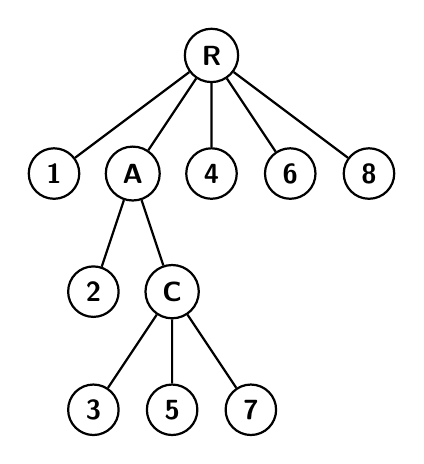
\begin{tikzpicture}[node distance=3cm,level distance=1.5cm,
                        level 1/.style={sibling distance=1cm},
                        level 2/.style={sibling distance=1cm},
                        thick,main node/.style={circle,draw,font=\sffamily\bfseries}]

    % Define vertices
    \node[main node] (R) {R}
        child {node[main node] (1) {1}}
        child {node[main node] (A) {A}
        child {node[main node] (2) {2}}
        child {node[main node] (C) {C}
        child {node[main node] (3) {3}}
        child {node[main node] (5) {5}}
        child {node[main node] (7) {7}}
        }
        }
        child {node[main node] (4) {4}}
        child {node[main node] (6) {6}}
        child {node[main node] (8) {8}}
        ;

    \end{tikzpicture}
    \caption{SCC Tree of Graph \ref{fig:graph1} after updates}
\end{subfigure}
\caption{Tree updates are propogated, deleting edge 4 to 8}
\label{fig:scc_tree_after_update_propogation2}
\end{figure}

\begin{algorithm}[H]
    \SetAlgoLined
    \KwData{Input data}
    \KwResult{Output result}
    initialization\;
    \While{termination condition is not met}{
        perform action\;
        update state\;
    }
    \caption{Example Algorithm}
\end{algorithm}

\begin{lstlisting}[language=C++, caption={Example C++ code}, label={lst:example_cpp_code}]
#include <iostream>

int main() {
    std::cout << "Hello, world!" << std::endl;
    return 0;
}
\end{lstlisting}